\section{Implementation}
\label{sec:implementation}

The implementation of \algst consists of a type checker and an interpreter, both
written in Haskell. Aiming at supporting more realistic programs, the
implementation features pragmatic extensions, including extensions to the
formal system and a simple module system for name space management.

\paragraph{Type checking}
\label{sec:type-checking}


The syntax of the implementation closely matches
the examples in this paper. Some places need additional kind annotations
because 
the type system of the implementation is not restricted to linear types. Its kind structure distinguishes
between linear and unrestricted variants of the kinds $\kinds$ and $\kindt$. Subkinding
allows us to subsume unrestricted versions of types to linear ones, that is, $\kindtu < \kindtl$. This subkinding generates a 
simple subtyping relation that essentially allows us to provide an unrestricted value where a linear
one is expected. The protocol kind $\kindp$ does not split in two versions, but still any type can be lifted to a protocol
type. \citet{DBLP:journals/corr/abs-2106-06658} investigate the metatheory of a system with a
similar kind structure (without the kind $\kindp$).


The type checker implementation closely follows the bidirectional
rules given in the paper. It necessarily contains an implementation of the type
normalization algorithm shown in \cref{fig:normalisation}. This
algorithm is extended to cater for the type isomorphism $\forall
\alpha. (T \to U) \cong T \to \forall \alpha.U$ (if $\alpha$ not free in $T$).  In this way, type applications can
be placed more liberally as long as their sequence is preserved.

The normalization algorithm is invoked exactly as indicated by the
algorithmic typing rules in \cref{fig:alg-typing}. By design, the
rules keep the typing assumptions and the outcome of inference in
normal form to minimize the number of times normalization is invoked.

The type checker includes further checking rules to enable writing some lambda abstractions without
type annotations. These rules are adaptions of well-known rules
\cite{DBLP:journals/csur/DunfieldK21}. For example:
\begin{mathpar}
  \infrule{\rulenameexpAbsn}
  {\expAgainst{\Gamma_1, \ebind xT}{e}{U}{\Gamma_2} \\ \termc{x}\not\in\Gamma_2}
  {\expAgainst{\Gamma_1}{\absne xTe}{\TFun[]{T}{U}}{\Gamma_2}}

  \infrule{\rulenameexpAppn}
  { \expSynth{\Gamma_1}{e_2}{T}{\Gamma_2}\\
   \expAgainst{\Gamma_2}{e_1}{\TFun[]{T}{U}}{\Gamma_3}} 
  {\expAgainst{\Gamma_1}{\appe {e_1}{e_2}}{\typec U}{\Gamma_3}}
\end{mathpar}

The implementation fully supports the overloaded use of data
constructors as protocol operators. We can perform pattern matching against the constructors of
a \lstinline+List+ datatype and use the same constructors in selecting alternatives of the
\lstinline+!List+ protocol. Moreover, the \lstinline+case+ operator is also overloaded to serve as
the \lstinline+match+ operator.



% The operations \lstinline+wait+ and \lstinline+terminate+ are not supported in
% the implementation. Instead, an exhausted channel is an unrestricted value of
% type \lstinline+End+ which can be discarded freely as it is not necessary to
% explicitly close a connection.

\paragraph{Interpretation}
\label{sec:interpretation}

The interpreter employs
standard techniques for the functional part and for
representing values at run time. 
It uses one universal type 
with constructors for each type in the language.
Processes in \algst are mapped to
Haskell threads. A fork in the language is implemented
using \texttt{forkIO} in Haskell. The interpreter is invoked recursively
for the new thread.

Communication channels are implemented using shared-memory abstractions from
Haskell's \texttt{Control.Concurrent} library. Synchronous
communication (as in this paper) is implemented
by pairs of \texttt{MVar}s, a semaphore-like concurrent datastructure
\cite{DBLP:conf/popl/JonesGF96} that behaves like a buffer of size
one. The implementation has an option to switch to
asynchronous channels using bounded
queues (\texttt{TBQueue}) from the \texttt{stm} library.

As channels are implemented in shared memory, the 
\lstinline|send| primitive is naturally polymorphic. Internally, the interpreter mediates
values of the universal type mentioned above between \lstinline+send+ and
\lstinline+receive+ operations.

\label{sec:benchmarking}
\begin{figure}[tp]
\begin{lstlisting}[morekeywords={rec},moreemph={End}]
--- protocol and type in AlgST syntax ---
protocol Repeat x = More x (Repeat x) | Quit
?Repeat Int . !(Char, EndT) . EndT
--- corresponding type in FreeST syntax ---
(rec repeat0 : 1S . &{More : ?Int ; repeat0 ; Skip,
                      Quit : Skip}) ; (!(Char, End) ; End)
--- example of an equivalent AlgST type ---
Dual (!Repeat Int . ?(Char, EndT) . Dual EndT)
--- example of a non-equivalent AlgST type ---
?Repeat String . !(Char, EndT) . EndT
\end{lstlisting}
  \caption{An \algst type instance, its FreeST counterpart and examples of equivalent and non-equivalent \algst types, following the rules of our test suite generator.}
  \label{fig:generated-example}
\end{figure}

\paragraph{Benchmarking}

We substantiate our claim that replacing a worst-case superlinear algorithm for
type equivalence by a linear one yields actual run-time improvements with an experiment.
We compare \algst's type equivalence algorithm with
FreeST, a freely available~\cite{FreeST-Language} programming language
containing an implementation of type equivalence for polymorphic
context-free session types
\cite{DBLP:conf/tacas/AlmeidaMV20,DBLP:journals/corr/abs-2106-06658}.
% \footnote{Available from
%   \url{http://rss.di.fc.ul.pt/tools/freest/}.}
As the type checker regularly requires type equivalence checks, the performance
of the equivalence algorithm should be understood as a lower
bound of the type checker performance.

To create a collection of equivalent and non-equivalent test cases, we 
implemented a generator of instances of \algst types. 
An instance comprises a set of mutually recursive algebraic protocols and a session type 
referring to them. We carefully restrict protocols and types
so that a translation from \algst instances to FreeST types is
possible: the generator avoids polymorphic and nested recursion and restricts the
occurrences of the negation operator to the top level of protocol
constructor arguments. 
For each instance $\typec{T}$, we randomly apply the properties of normalization 
to generate 
an equivalent \algst type $\typec{T'}$ (see~\cref{fig:normalisation}). The pairs 
$(\typec{T}, \typec{T'})$ constitute our test suite of equivalent types. 
Non-equivalent tests are obtained from each $\typec{T}$ 
by either introducing an additional quantifier, or changing a sub-part of the
type to something of the same kind. Possible
replacements are the quantified type variables and the types built into AlgST,
such as \lstinline+Int+ or \lstinline+String+. The \algst type is
translated to a session type in FreeST. Protocols are translated inline at
every point of use as recursive branch or choice types, depending on wether it
appears in a sending or receiving context.
For single constructor types, the translation omits the constructor
tag. The arguments of the constructors are translated into nested
sequences of single interactions. See \cref{fig:generated-example} for an example.

Benchmarks were run using the gauge package v0.2.5 \cite{gauge} with a
timeout of 2~minutes. AlgST was compiled using GHC 9.2.7, FreeST used GHC 8.10.7.
Each test suite comprises 324 tests. FreeST incurred 69 timeouts for the positive tests and 77 timeouts for the negative tests.
\Cref{fig:timings} compares the execution time of the \algst and FreeST type equivalence algorithms 
for the equivalent and non-equivalent test cases. 
%(\cref{fig:time-positiv} and \ref{fig:time-negative}, resp.). 
% The plots are presented in log scale and vary with the number of nodes of the \algst type in the abstract syntax tree.
The plots substantiate the differences in the execution time of FreeST and \algst, distinguishing the 
linear evolution of \algst and 
the exponential behavior of FreeST as a function of the number of nodes in the abstract
syntax tree of the AlgST type. 
%The plots are represented in log scale.

\begin{figure}[tp]
  \begin{subfigure}{.5\textwidth}
    \centering
    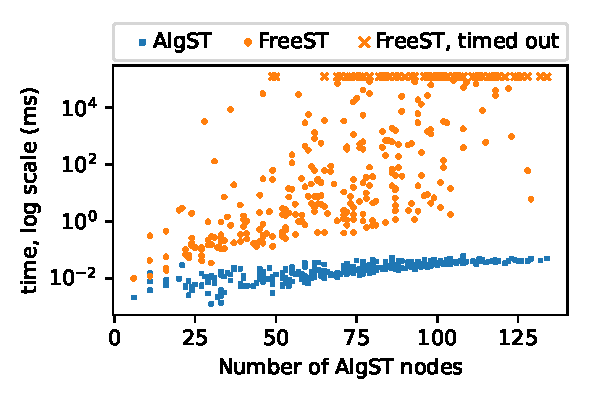
\includegraphics[width=\linewidth]{img/fig-pos.pdf}
    \caption{equivalent test cases}
    \label{fig:time-positiv}
  \end{subfigure}%
  \begin{subfigure}{.5\textwidth}
    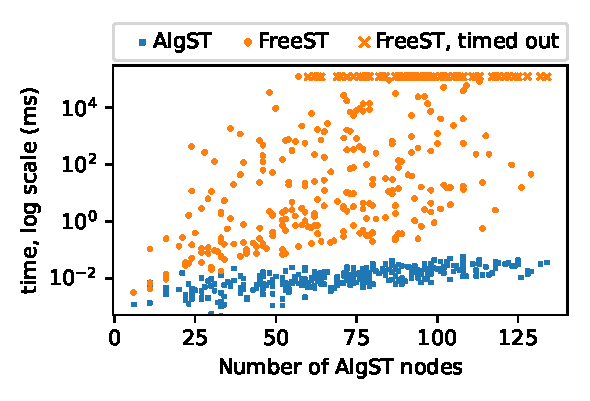
\includegraphics[width=\linewidth]{img/fig-neg.pdf}
    \caption{non-equivalent test cases}
    \label{fig:time-negative}
  \end{subfigure}
  \caption{Execution time of the \algst and FreeST type equivalence algorithms on the equivalent and non-equivalent test cases, represented in log scale as a function of the number of \algst nodes in the AST.}
  \label{fig:timings}
\end{figure}

%%% Local Variables:
%%% mode: latex
%%% TeX-master: "main"
%%% End:
